%% LaTeX Beamer presentation template (requires beamer package)
%% see http://bitbucket.org/rivanvx/beamer/wiki/Home
%% idea contributed by H. Turgut Uyar
%% template based on a template by Till Tantau
%% this template is still evolving - it might differ in future releases!

\documentclass{beamer}

\mode<presentation>
{
\usetheme{Warsaw}

\setbeamercovered{transparent}
}

\usepackage[french]{babel}
\usepackage[utf8]{inputenc}
\usepackage{graphicx}
\usepackage{listings}

% font definitions, try \usepackage{ae} instead of the following
% three lines if you don't like this look
\usepackage{mathptmx}
\usepackage[scaled=.90]{helvet}
\usepackage{courier}


\usepackage[T1]{fontenc}



\title{Éco-conception de logiciels}

\subtitle{Soutenance de stage de 5ème année}

% - Use the \inst{?} command only if the authors have different
%   affiliation.
%\author{F.~Author\inst{1} \and S.~Another\inst{2}}
\author{Guillaume Delamare}

% - Use the \inst command only if there are several affiliations.
% - Keep it simple, no one is interested in your street address.
\institute[Universities of]
{
%
\includegraphics[width=0.25\textwidth]{figures/logo-emn.jpg}
Équipe ASCOLA\\
Laboratoire d'informatique de Nantes Atlantiques\\
École des Mines de Nantes\\
}

\date{\today}

% This is only inserted into the PDF information catalog. Can be left
% out.
\subject{Talks}

% If you have a file called "university-logo-filename.xxx", where xxx
% is a graphic format that can be processed by latex or pdflatex,
% resp., then you can add a logo as follows:

\pgfdeclareimage[height=0.5cm]{university-logo}{figures/logo-emn}
\logo{\pgfuseimage{university-logo}}

% Delete this, if you do not want the table of contents to pop up at
% the beginning of each subsection:
\AtBeginSection[]
{
\begin{frame}<beamer>
\frametitle{Plan}
\tableofcontents[currentsection,hideothersubsections]
\end{frame}
}

% If you wish to uncover everything in a step-wise fashion, uncomment
% the following command:

%\beamerdefaultoverlayspecification{<+->}

\begin{document}

	\begin{frame}
		\titlepage
	\end{frame}

	\section*{Introduction}
		\begin{frame}
			\frametitle{Plan}
			\tableofcontents[hideallsubsections]
		\end{frame}

	\section{Contexte du stage}
		\subsection{Lieu de stage}
			\begin{frame}
				\frametitle{L'équipe ASCOLA}
				\begin{itemize}
					\item Installé au département informatique de l'école des Mines de Nantes
					\item Fait partie du LINA et de l'INRIA 
				\end{itemize}
			\end{frame}
			
		\subsection{Sujet de stage}
			\begin{frame}
				\frametitle{Sujet}
					\begin{block}{Le context}
						Toujours plus d'équipements informatiques, toujours plus complexe, plus couteux, et plus consommateur en énergie.
					\end{block}
					\begin{block}{Le sujet}
						Réduire la consommation des systèmes d'informations  en travaillant sur la conception du logiciel.
					\end{block}
			\end{frame}
			\begin{frame}
				\frametitle{Objectifs}
				
				Définir des techniques, des patterns et des outils pour rendre moins énergivore les logiciels
			    \begin{block}{Pour cela, il faut :}
				    \begin{itemize}
						\item Identifier les travaux réalisés dans le domaine
						\item Mettre au point une méthodologie permettant de quantifier l'énergie consommée
						\item Faire des propositions et les expérimenter
				    \end{itemize}
			    \end{block}
			\end{frame}
		
	\section{État de l'art}
		\subsection{Mesure de la consommation d'énergie}
			\begin{frame}
				\frametitle{L'outil de base : le wattmètre}
				\begin{center}
					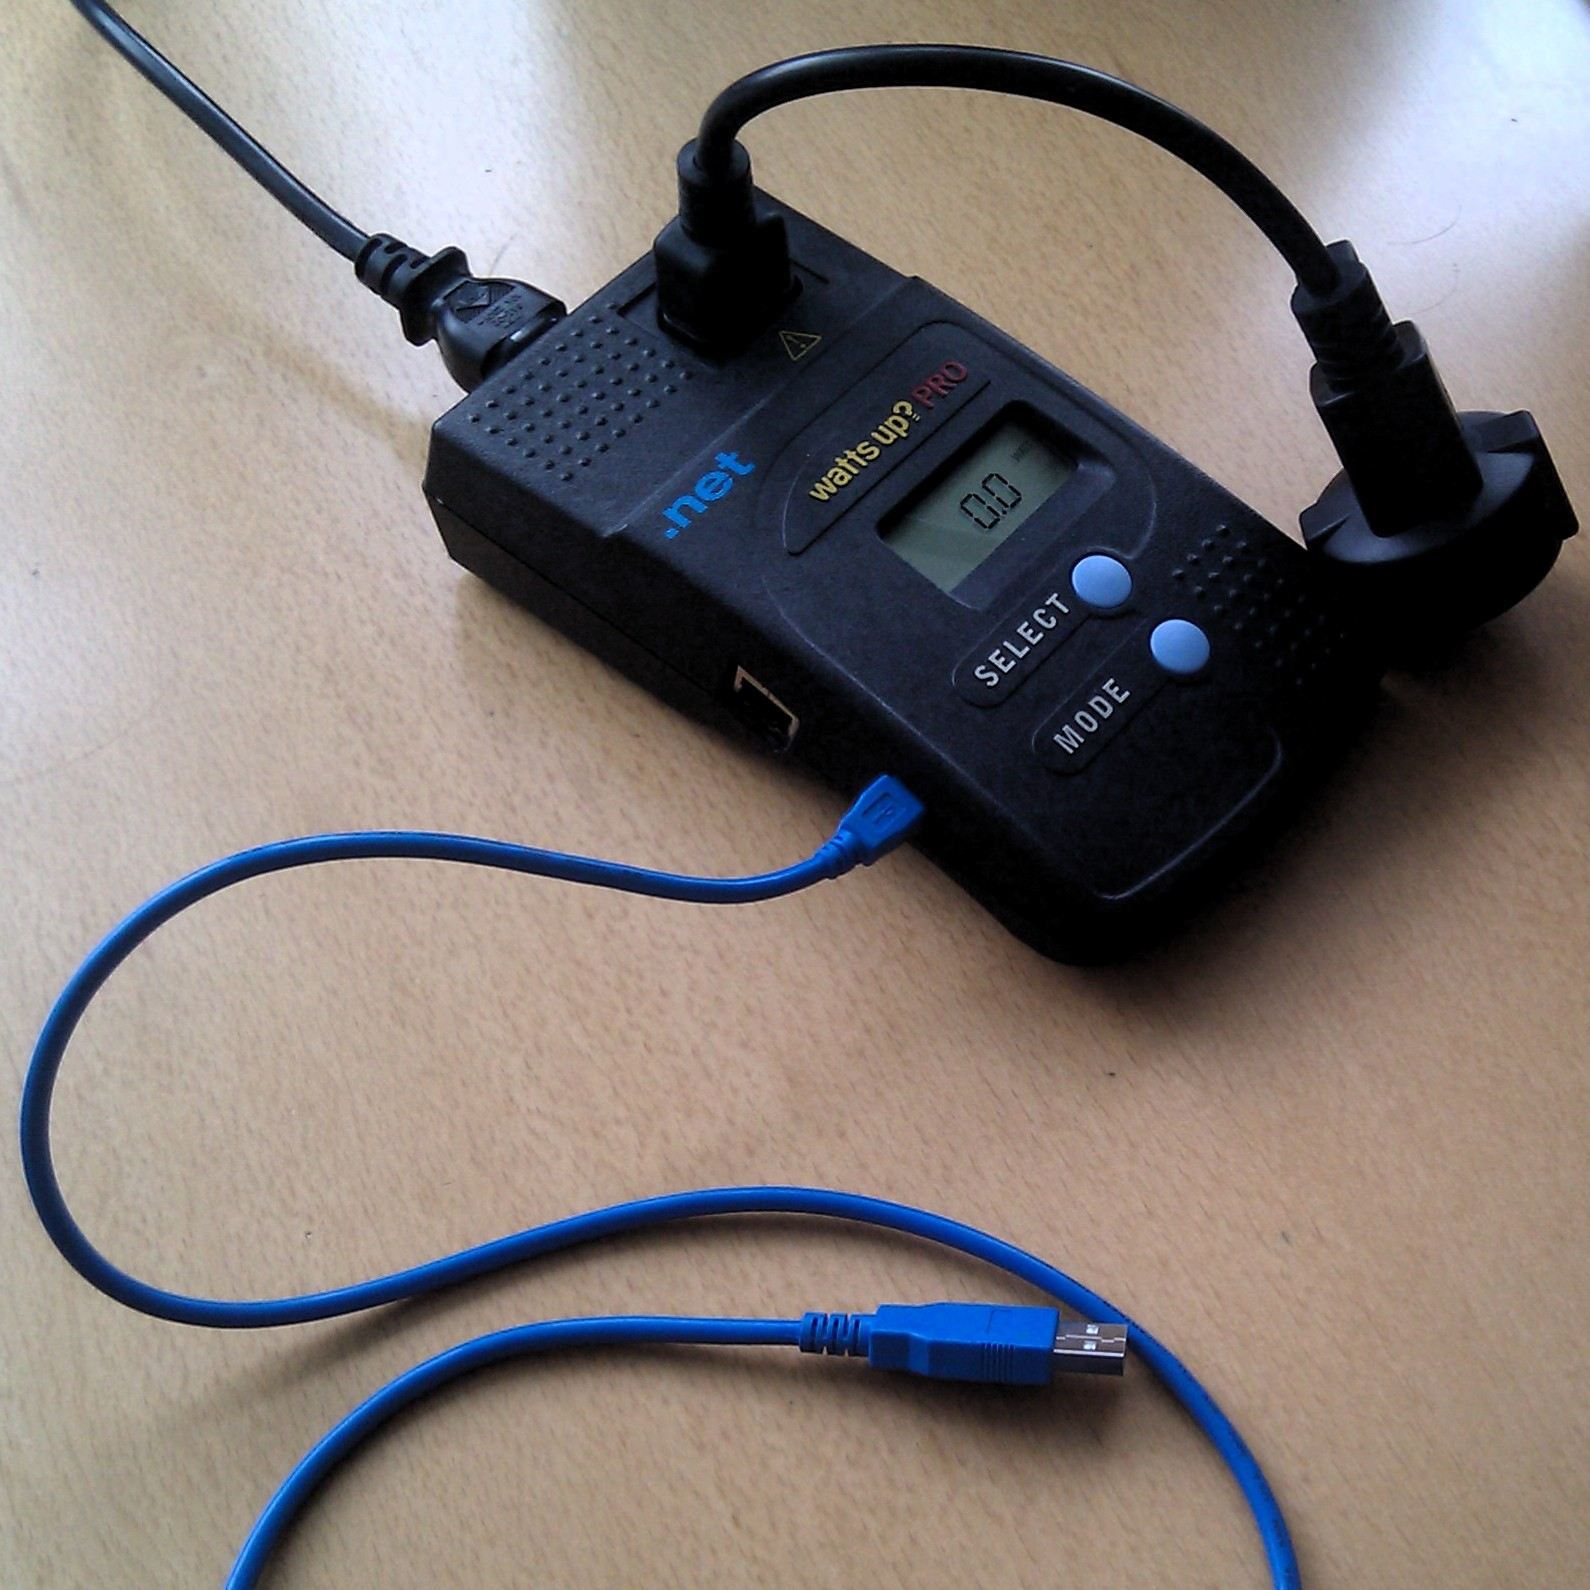
\includegraphics[width=0.50\textwidth]{figures/wattsup}
				\end{center}
			\end{frame}
			\begin{frame}
				\frametitle{Mesure logiciel de la consommation}
					On peut estimer la consommation d'un logiciel à partir d'informations fourni par le système. Pour cela il faut :
					\begin{itemize}
						\item Mesurer les ressources consommées par le logiciel
						\item Transformer ces mesures en consommation au moyen d'un modèle
					\end{itemize}
					L'enjeu est donc d'avoir un modèle adapter pour la machine sur laquelle fonctionne le logiciel 
			\end{frame}
			\begin{frame}
				\frametitle{Et dans le futur ?}
					\begin{itemize}
						\item Des sondes directement installées sur les composants d'une machine.
						\item Des API fournit par les constructeurs pour récupérer les mesures.
					\end{itemize}
			\end{frame}
			
		\subsection{Bonnes pratiques}
			\begin{frame}
				\frametitle{Conception}
					\begin{block}{L'exemple du Green Challenge}
						Les gagnants on choisi :
						\begin{itemize}
							\item De déplacer les traitrements coté serveur
							\item D'évaluer le coup des Bibliothèques utilisées
							\item D'éviter certain langage
						\end{itemize}
					\end{block}
			\end{frame}
			\begin{frame}
				\frametitle{Programmation}
					
			\end{frame}
			
		\subsection{Travaux connexes}
			\begin{frame}
				\frametitle{Travaux connexes}
				\begin{block}{Quelques projets connexes}
					\begin{itemize}
						\item Le Projet code vert
						\item Le Green code Lab
					\end{itemize}
				\end{block}
			\end{frame}
		
	\section{Contributions}
		\subsection{Test des outils de mesure}
			\begin{frame}
				\frametitle{Les échecs}
					\begin{block}{Deux projets inapropriés}
						\begin{itemize}
							\item Energy checker
							\item PTop
						\end{itemize}
					\end{block}
			\end{frame}
			\begin{frame}
				\frametitle{ClassMexer}
				
			\end{frame}
			\begin{frame}
				\frametitle{JouleMeter}
				\begin{center}
					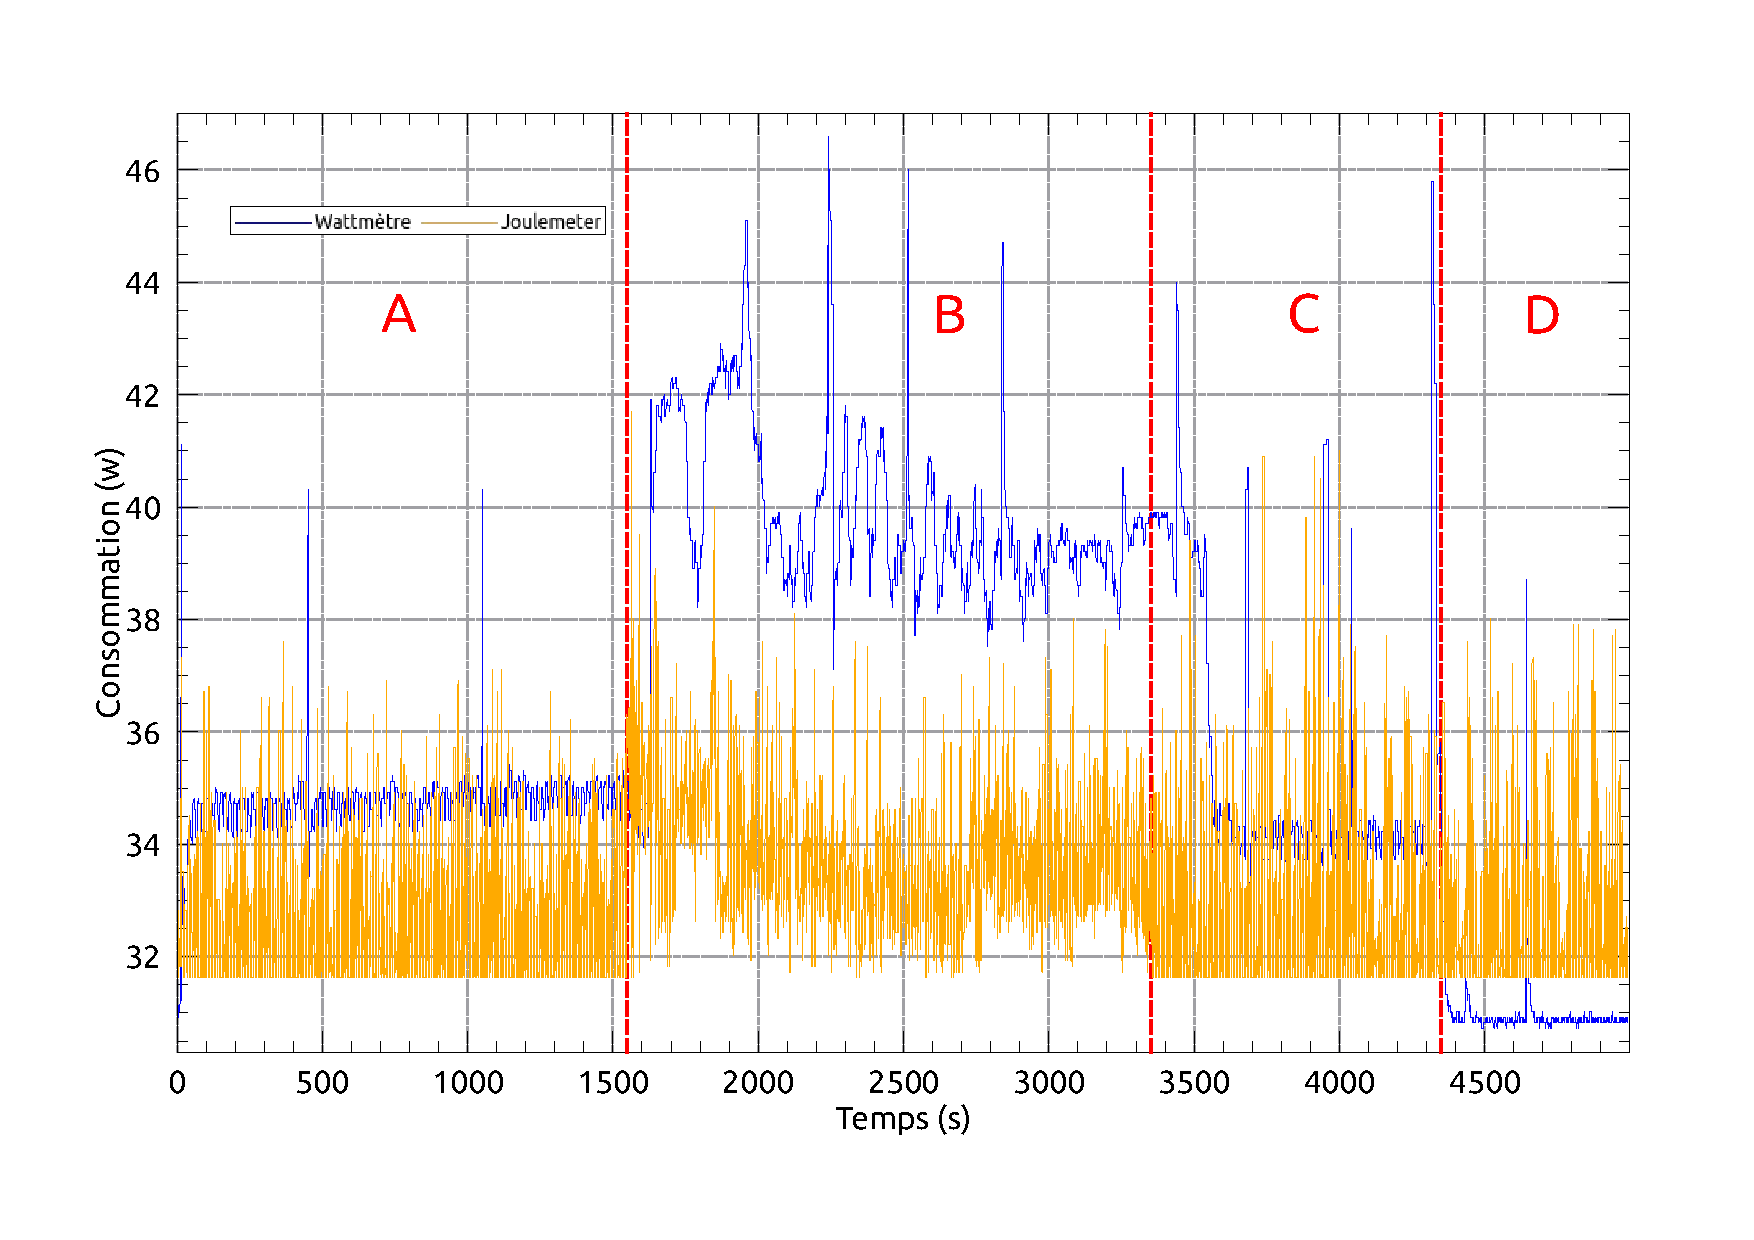
\includegraphics[width=0.8\textwidth]{figures/joulemeter}
				\end{center}
			\end{frame}
			\begin{frame}
				\frametitle{PowerAPI}
					\begin{itemize}
					  \item Développé par l'équipe ADAM de Lilles
					  \item Semble donner des résultats assez proche de la réalité
					\end{itemize}
			\end{frame}
			
		\subsection{OSGi pour économiser l'énergie}
			\begin{frame}
				\frametitle{Présentation d'EcoFramework}
					\begin{block}{Objectifs}
						\begin{itemize}
						  \item Une architecture modulaire
						  \item Un système permettant la dégradation de service
						  \item Remplacer du code gourmand par un plus économe
						\end{itemize}
					\end{block}
			\end{frame}
			\begin{frame}
				\frametitle{Présentation d'EcoFramework}
				\begin{center}
					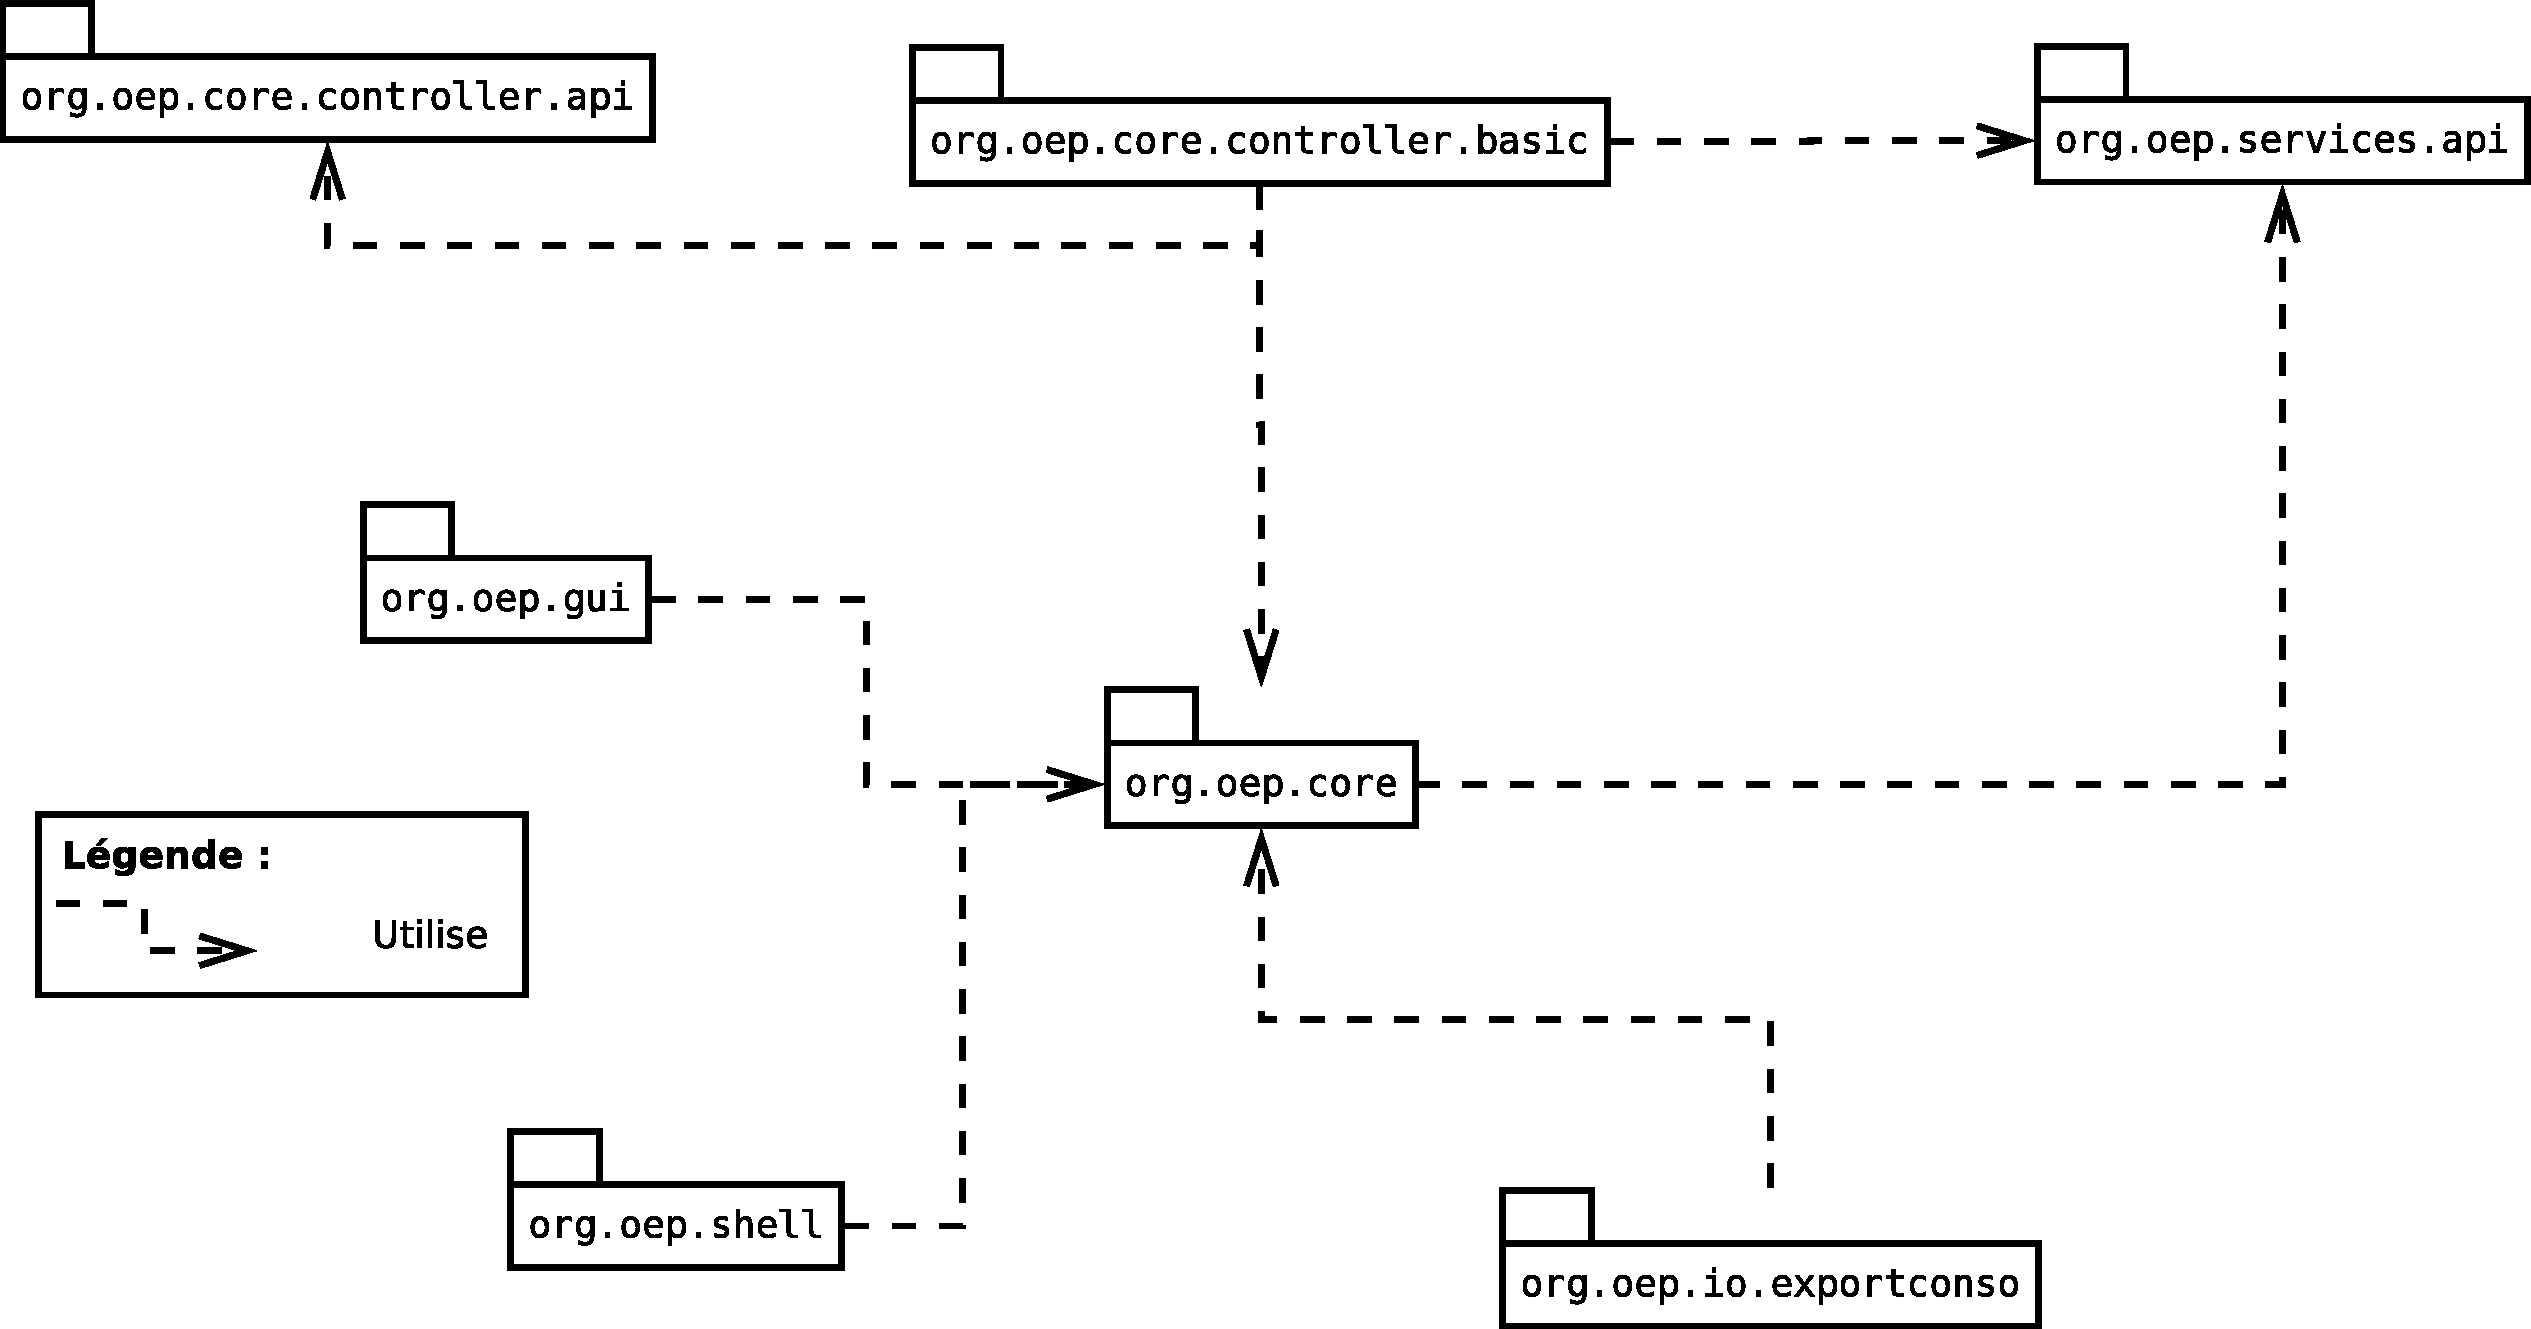
\includegraphics[width=0.8\textwidth]{figures/EcoPattern_Bundle_Diagramme.pdf}
				\end{center}
			\end{frame}
			\begin{frame}
				\frametitle{Exemple d'application : Lecteur multimedia}
				\begin{center}
					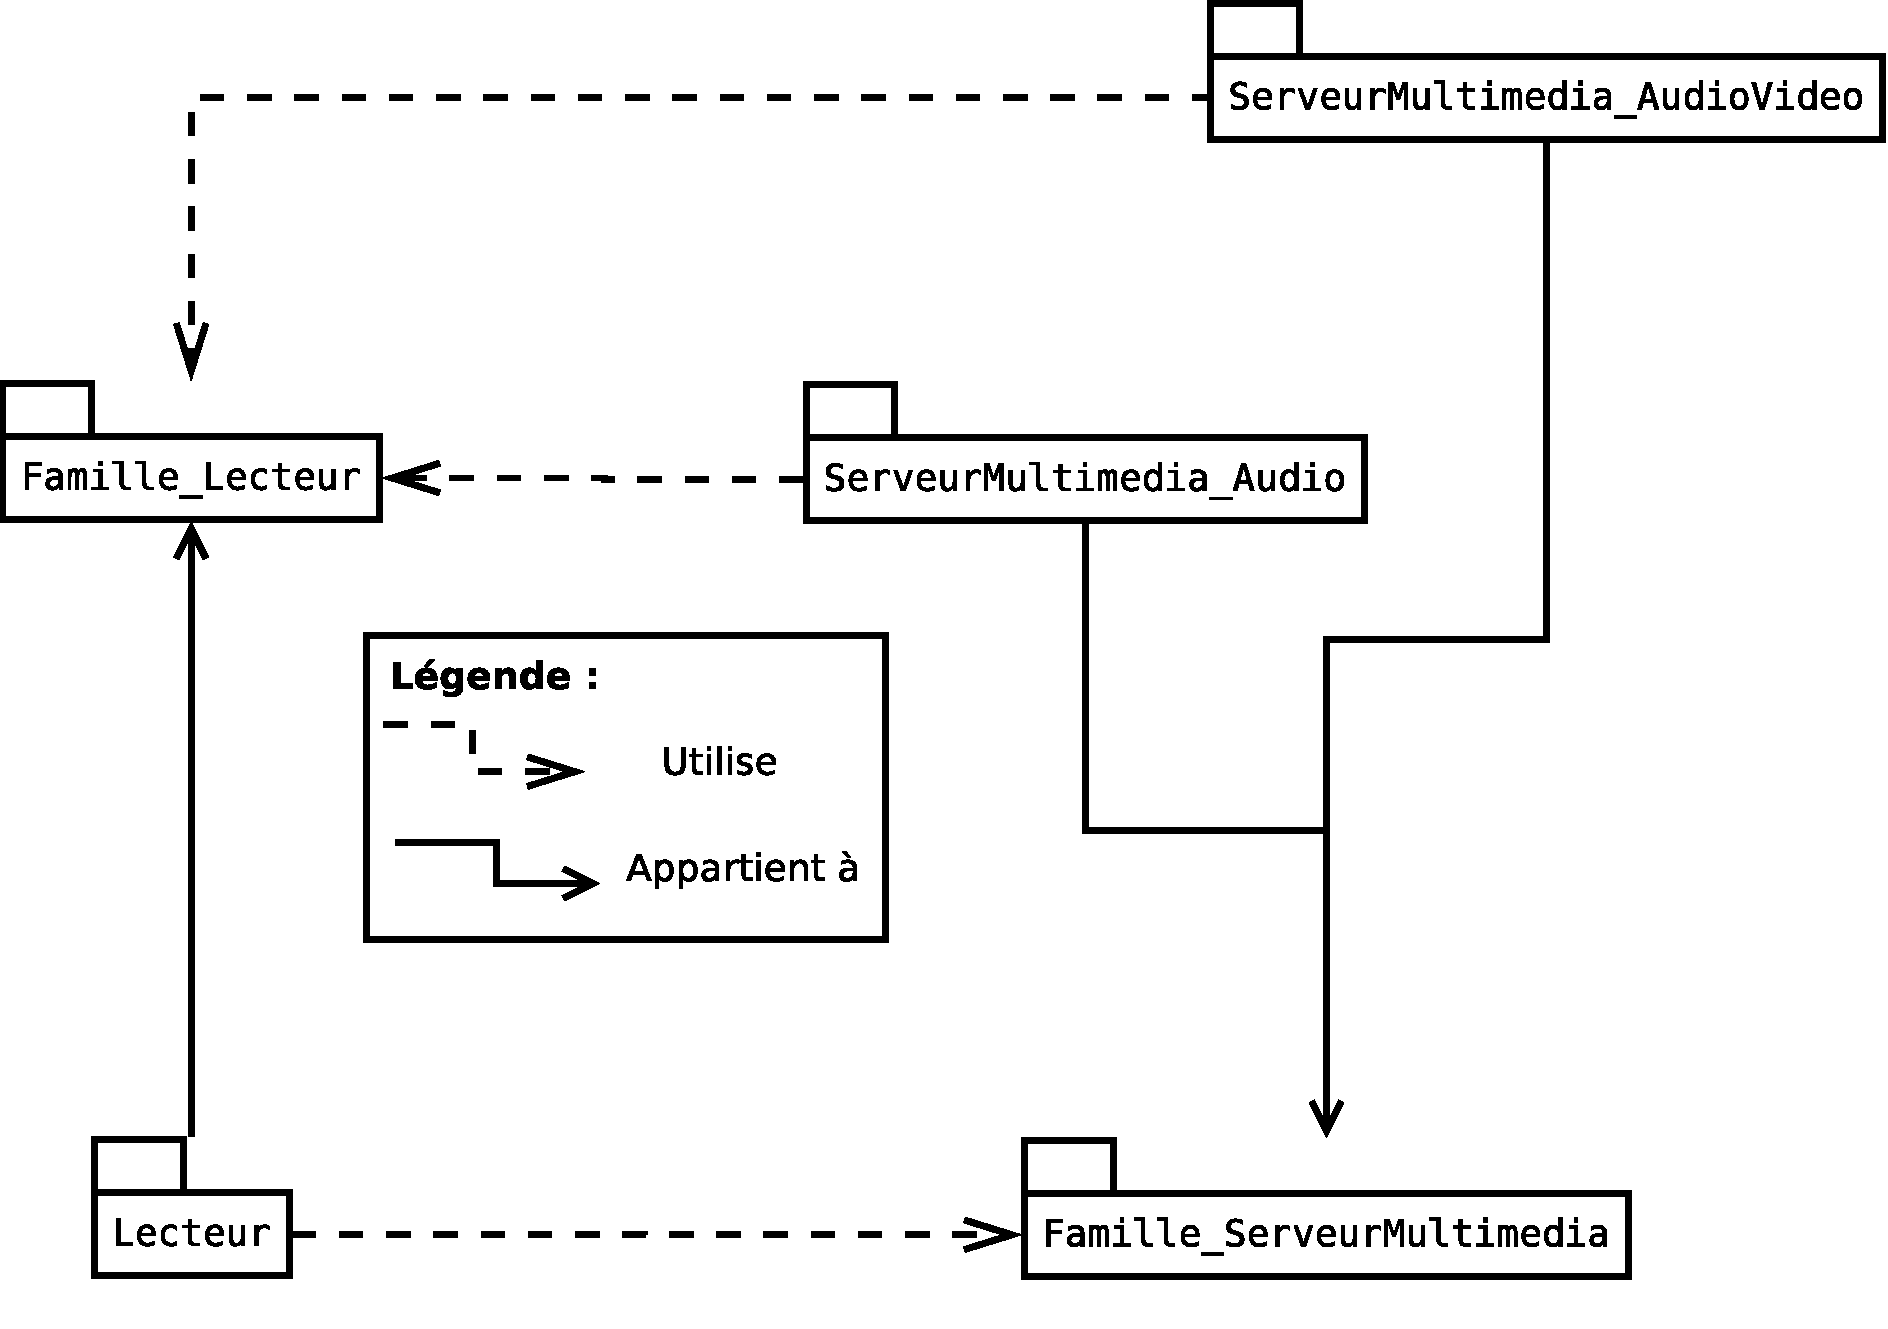
\includegraphics[width=0.8\textwidth]{figures/EcoPattern_LecteurMultimedia.pdf}
				\end{center}
			\end{frame}
			\begin{frame}
				\frametitle{Démonstration}
				
			\end{frame}
			
	\section{Conclusion}
		\begin{frame}
			\frametitle{Conclusion}
			\begin{itemize}
			  \item Un stage passionnant, riche en découverte et apprentissage
			  \item Des conditions de travail idéal
			  \item Un sujet à peine ouvert 
			\end{itemize}
		\end{frame}
		\begin{frame}
			\frametitle{Questions}
				Avez vous des Questions ?
		\end{frame}
\end{document}